
\chapter{Algoritmo BRKGA con búsqueda local para TOP}

En el presente capítulo ahondaremos en detalle la solución implementada para el \textit{Team Orienteering Problem}. La implementación se la puede dividir en 3 módulos importantes. Primero el decodificador, que como mencionamos en el capítulo BRKGA tiene la tarea de convertir un arreglo de enteros aleatorios en una solución válida del problema. Luego el algoritmo BRKGA, cuya implementación puede hacerce con total independencia del problema a resolver. Por último las heurísticas locales aplicadas en cada nueva generación a el mejor individuo de la población, al cual no se le hayan aplicado previamente. 

\bigskip

En el capítulo \textit{Resultados} se mostrara en detalle los resultados obtenidos de la versión final de la implementación sobre el benchmark de problemas de Chao y Tsiligirides \cite{IntancesChaoTsiligirides}. Se compararon los resultados con los obtenidos de los trabajos previos de Chao et al. \cite{ChaoGoldenWasil}, de Archetti et al. \cite{ArchettiHertzSperanza} y los de Tang and E. Miller-Hooks \cite{TangMillerHooks}. En este capítulo se utilizaran los resultados de tales trabajos previos para crear un índice de efectividad a modo de poder evaluar la efectividad de la solución generada por el modulo analizado.

\bigskip

Además contaré las dificultades encontradas y desiciones tomadas para llegar a soluciones más competitivas con los trabajos previos seleccionados. A modo de monitorear el progreso, primero se seleccionó un subconjunto diverso del benchmark de problemas de Chao y Tsiligirides \cite{IntancesChaoTsiligirides}. Luego, para cada versión de la implementación que fui generando, se les calculó su índice de efectividad. Tal índice lo definí de la siguiente manera:

\begin{equation*}
bestProfit(i) = Max(Profit(CGW(i)), Profit(AHS(i)), Profit(TMH(i)))
\end{equation*}
\begin{equation*}
efectividad(imp_{v.xyz}) = Profit(imp_{v.xyz}(i)) / bestProfit(i)
\end{equation*}

\bigskip

Donde $Profit(Implementacion_v.xyz(i))$ representa la ganancia de la mejor solución obtenida luego de ejecutar una cierta cantidad de veces la version $xyz$ para la intancia del problema $i$. Luego $Profit(CGW(i))$, $Profit(AHS(i)$, $Profit(TMH(i))$ representan la ganancia de las implementaciones de Chao et al., Archetti et al. y Tang Miller-Hooks respectivamente para la misma instancia $i$. El índice es simplemenete devidir la ganancia obtenida por la mejor ganancia encontrada por los trabajos previos seleccionados. Si el $efectividad(imp_{v.xyz}) = 1$, luego nuestra implementación habra generado una solución tan buena como los trabajos previos. Si $0.95 \leq efectividad(imp_{v.xyz}) < 1$, mi solución no sera tan buena pero considero que esta en un rango donde es  competitiva. A lo largo de todo el desarrollo, el objetivo fue maximizar el índice de efectividad sin tener certeza de llegar a buenas soluciones utlizando la heurística BRKGA.

\bigskip

Para cada uno de los siguientes modulos y submodulos, se mostraran su pseudocodigo y su índice de efectividad. El pseudocódigo utilizado sigue la sintaxis de c\#, el lenguaje en el cual implemente el desarrollo. El objetivo del pseudocodigo es meramente descriptivo, el método que representa puede ser implementado con ciertas variaciones que no viene al caso describir. Tales variaciones para no mostrar: variables de medición de tiempo, variables para monitorear estados, testing, manejo de excepciones, persistencia de resultados, y demas, con el objetivo de ser mas ilutrativo de la funcionalidad del algoritmo. 


\bigskip

Para la valuación del índice de efectividad se eligieron seis intancias del benchmark de modo que fueran variadas entre si. Tome dos pequeñas, dos medianas y dos grandes, cuyas descripción pueden observarse en la siguiente tabla:

\begin{center}
\begin{tabular}{ |c|c|c|c|c| } 
 \hline
Autor & Instancea & Vertices & Vehículos & TMax \\
\hline
Tsiligirides & p2.2.k & 21 & 2 & 22.50 \\
Tsiligirides & p2.3.g & 21 & 3 & 10.70 \\
Tsiligirides & p3.4.p & 33 & 4 & 22.50 \\
Chao & p5.3.x & 66 & 3 & 40.00 \\
Chao & p7.2.e & 102 & 2 & 50.00 \\
Chao & p7.4.t & 102 & 4 & 100.00 \\
 \hline
\end{tabular}
\end{center}


\bigskip

Las tablas donde mostraré el índice de efectividad de los resultados parciales tendrá un subconjunto de los siguientes encabezados:

\begin{center}
\begin{tabular}{ |c|c|c|c|c|c|c|c|c|c|c|c| } 
 \hline
$I$ & $\#N$ & $\#V$ & $tMax$ & $C$ & $\#S$ & $T_{avg}$ & $B_{max}$ & $B_{min}$ & $B_{avg}$ & $i_{f}$ & $BTP_{max}$ \\
\hline
\end{tabular}
\end{center}

\bigskip

Donde:\label{tableHeader}
$Profit(CGW(i))$, $Profit(AHS(i)$, $Profit(TMH(i))$
\begin{itemize}
	\item \textbf{$I$}: Nombre de la instancia. Ej: p2.3.g
	\item \textbf{$\#N$}: Cantidad de nodos de la instancia. Ej: 21
	\item \textbf{$\#V$}: Cantidad de vehículos de la instancia. Ej: 3
	\item \textbf{$tMax$}: Distancia máxima de la ruta de los vehículos de la instancia. Ej: 10.70
	\item \textbf{$C$}: Configuración general del BRKGA. Es un código que sintetisa la configuración basica global, explicado en detalla más adelante (ver sección \label{sec:descrCongif}).
	\item \textbf{$\#S$}: Cantidad de soluciones de las cuales se sacaron los datos. Ej: 200
	\item \textbf{$T_{avg}$}: Tiempo promedio en milisegundos de la ejecución total de la implementación. Ej: 21578
	\item \textbf{$B_{max}$}: Beneficio máximo de las \#S soluciones generadas. Ej: 140
	\item \textbf{$B_{min}$}: Beneficio mínimo de las \#S soluciones generadas. Ej: 45
	\item \textbf{$B_{avg}$}: Beneficio promedio de las \#S soluciones generadas. Ej: 45
	\item \textbf{$i_{f}$}: Indice de efectividad. Se utiliza el $B_{avg}$ para tener un valor que mejor refleje la efectividad real. Si usara $B_{max}$, el indice aparentaría muy bueno si entre las \#S soluciones se genero una muy buena aleatoriamente. Ej: $B_{avg} / BTP_{max} = 0.57$
	\item \textbf{$BTP_{max}$}: Beneficio de Trabajos Previos máximo para la misma instancia. Los trabajos previos utilizados son CGW, AHS y TMH. Ej: 145
\end{itemize}

\section{Decodificador}

El decodificador debe generar una solución valida del problema dado un vector aleatorio de enteros y conociendo la instancia del problema (vehículos disponibles, clientes, tmax, etc). A modo El decodificador construye una solución valida asignando clientes a las rutas de los vehículos disponibles respetando tmax, su distancia maáxima de recorrido. El orden en que toma los clientes a asignar es clave y determina la solución resultante. Es ahí donde utilizaremos el vector aleatorio de enteros, el vector aleatorio de enteros marcara el orden en el cual se tomaran los clientes para asignarlos a una ruta. Por lo tánto el vector aleatorio de enteros tendrá una longitud equivalente a la cantidad de clientes del problema (vertices con beneficio mayor a cero).

\subsection{Orden de los clientes a considerar}\label{sec:ordenDeco}

Dado una instacia de un problema con $n$ clientes y un vector de enteros aleatorio de tamaño $n$, un decoder genera una solución valida de un problema. El vector, en mi implementacion, es un vector de RandomKeys. Un $RandomKey$ tiene dos propiedades, el entero aleatorio llamado $Key$ y otro entero llamado $PositionIndex$. 

\bigskip

\begin{lstlisting} 
public class RandomKey
{        
	public int Key { get; private set; }
	public int PositionIndex { get; private set; }
}
\end{lstlisting}

\bigskip

El propositio de $PositionIndex$ es para mapear un Key con un Cliente. Existe un arreglo de clientes en el Mapa del problema. Los clientes siempre tienen la misma posicion y esa posicion es un entero en el intervalo $[0, \#Clientes-1]$. Luego para un vector de RandomKeys de tamaño $\#Clientes$ no existen dos RandomKeys con mismo valor de PositionIndex y todos los PositionIndex se encuentran en el itervalo $[0, \#Clientes-1]$. De forma que cada RandomKey matchea siempre con solo RandomKey. Luego se matchean los clientes con los randomKeys por su position index y se los ordena de forma ascendente por el Key aleatorio. Esto se puede ver en la figura \ref{fig:RandomKeysOrdenando}.

\bigskip

\begin{lstlisting} 
public List<Client> GetOrderedClients(List<RandomKey> randomKeys)
{        
	return randomKeys.OrderBy(r => r.Key).Select(r => Map.Clients[r.PositionIndex]);
}
\end{lstlisting}

\begin{figure}[h]
	\caption{RandomKeys ordenando clientes}
	\centering
	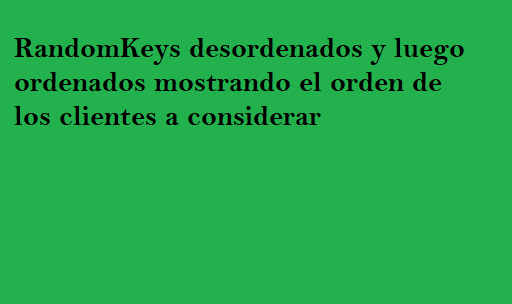
\includegraphics{RandomKeysOrdenando}
	\label{fig:RandomKeysOrdenando}
\end{figure}

\subsection{Decodificador simple}

El decodificador simple recibe como parametro el vector de enteros aleatorios y con eso genera los clientes ordenados. Luego por cada vehiculo, si el siguiente cliente se puede incluir en la ruta se incluye sino considera que la ruta esta completa y pasa al siguiente vehiculo. Un cliente $c_i$ se puede agregar a la ruta si al agregarlo no supera la distancia maxima permitida para la ruta. Sean $v$ vehiculo, $dMax$ la distancia maxima de $v$, $dAct$ la distancia actual de $v$, $f$ el destino final de la ruta, $c_u$ el ultimo cliente agregado a la ruta de $v$ y $c_i$ cliente a evaluar agregar a la ruta de $v$. Luego cree la funcion can visit que implementa la siguiente formula:

\bigskip

\( dAct\, +\, distancia(c_u, c_i)\, +\, distancia(c_i, f)\, -\, distancia(c_u, f) \leq dMax\)

\bigskip

Pseudocodigo del método decode del decodificador simple:

\bigskip

\begin{lstlisting} 
public Solution Decode(List<RandomKey> randomKeys, ProblemInfo pi)
{
	var clients = GetOrderedClients(randomKeys);
	var vehicles = pi.GetVehicles();	
	var iv = 0;
	var ic = 0;	
	do
	{
		if(vehicles[iv].CanVisit(clients[ic]))
		{
			vehicles[iv].AddClient(clients[ic]);
			ic++;
		}
		else
		{
			iv++;			
		}
		
	} while(iv < vehicles.Length && ic < clients.Length)	
	var solution = pi.InstanceSolution(vehicles);
	return problem;
}
\end{lstlisting}

A partir de 200 $RandomKeys$ generé 200 soluciones con el decoder simple para las subconjunto de instancias diversas elegidas. Se utilizaron distintos sets de 200 $RandomKeys$ para cada instancia. La siguiente tabla tiene los resultados obtenidos (ver \ref{tableHeader} para significado de columnas):

\begin{center}
\begin{tabular}{ |c|c|c|c|c|c|c|c|c|c| } 
\hline
$I$ & $\#N$ & $\#V$ & $tMax$ & $\#S$ & $B_{max}$ & $B_{min}$ & $B_{avg}$ & $i_{f}$ & $BTP_{max}$ \\
\hline
p2.2.k & 21 & 2 & 22.50 & 200 & 175 & 40 & 102 & 0.37 & 275  \\
p2.3.g & 21 & 3 & 10.70 & 200 & 140 & 45 & 83 & 0.57 & 145  \\
p3.4.p & 33 & 4 & 22.50 & 200 & 270 & 90 & 170 & 0.30 & 560  \\
p5.3.x & 66 & 3 & 40.00 & 200 & 405 & 195 & 295 & 0.19 & 1555  \\
p7.2.e & 102 & 2 & 50.00 & 200 & 98 & 8 & 39 & 0.13 & 290  \\
p7.4.t & 102 & 4 & 100.00 & 200 & 221 & 40 & 116 & 0.11 & 1077  \\
\hline
\end{tabular}
\end{center}

En estos resultados ya se puede observar una correlación que sera recurrente, para intancias pequeñas los resultados son mejores.

\subsection{Caracteristicas y debilidades del decodificador simple}

Tiene un orden de complejidad de $O(\#clientes)$.

\bigskip

Sea $v$ el vector de clientes ordenados por un vector aleatorio de enteros. Existen $m+1$ indices $i_0 = 0, i_1, i_2, .., i_m$ donde $m$ es la cantidad de vehículos y $0 \leq i_j \leq \#clientes$ tales que el vehículo $j$ incluye en su recorrido a todos los clientes del subvector $v[i_{j-1}, i_j-1]$. Luego todos los clientes en el subvector $v[i_m, v.Length - 1]$ son clientes no alcanzados por la solucion. Esto puede verse en la figura \ref{fig:DistribucionClientesDecoSimple}.

\begin{figure}[h]
	\caption{Marcados con un color por vehiculo como quedan los clientes distribuidos con el decoder simple}
	\centering
	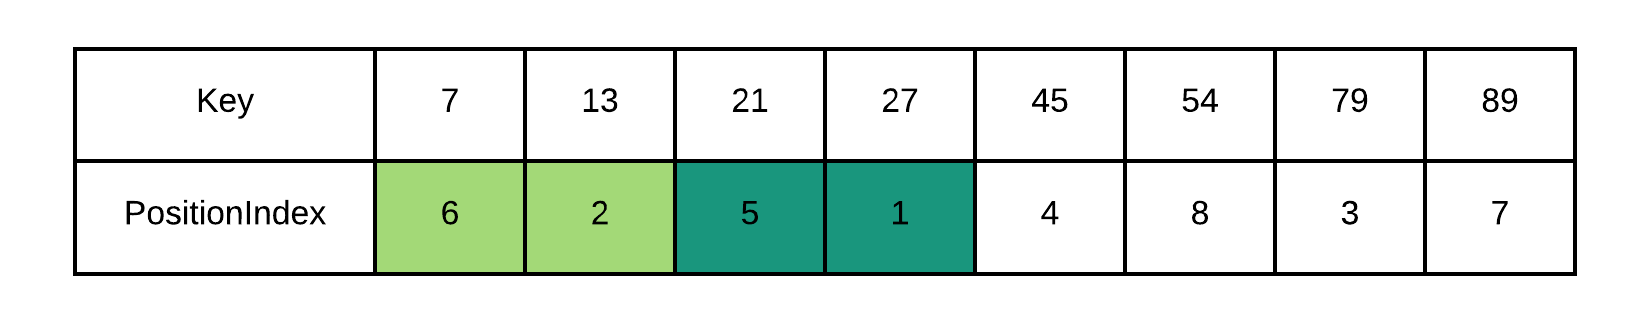
\includegraphics{DistribucionClientesDecoSimple}
	\label{fig:DistribucionClientesDecoSimple}
\end{figure}

\bigskip

Un problema que tiene este decodificar es en la existencia de un cliente inalcansable, es decir si existe $c$ cliente tal que:

\( distancia(i, c)\, +\, distancia(c, f)\, >\, dMax\)

Esto puede generar soluciones de la poblacion donde existan vehiculos con rutas vacias. La solucion facil a este problema es filtrando todos los clientes inalcansables previo a la ejecucion del BRKGA.

\bigskip

Otro problema que tiene este decodificador es que cambia de vehiculo al primer intento fallido de expandir su ruta. Luego puede generar soluciones con rutas muy pequeñas, por este motivo implemente un Decodificador Goloso.


\subsection{Decodificador Goloso}

El decodificador goloso en principio funciona igual que el decodificador simple hasta que llega a un cliente que no pudo agregar a la ruta de un vehículo. En este caso, en vez de pasar a trabajar con el siguiente vehículo disponible, intenta agregar al siguiente cliente y así sucesivamente hasta que no hay mas clientes que intentar. Luego al pasar al siguiene vehiculo intenta solamente con los clientes no asignadas a los vehículos anteriores y siempre respetando el orden de los clientes asignado por el vector de enteros aleatorios.

\bigskip

\begin{lstlisting} 
public Solution Decode(List<RandomKey> randomKeys, ProblemInfo pi)
{
	var clients = GetOrderedClients(randomKeys);
	var cIterator = new Iterator(cliets);
	var vehicles = pi.GetVehicles();	
	var iv = 0;
	while(iv < vehicles.Length)
	{
		while(!cIterator.IsEmpty)
		{
			if(vehicles[iv].CanVisit(cIterator.Current))
			{
				vehicles[iv].AddClient(cIterator.Current);
				cIterator.RemoveCurrent;
			}
			else
			{
				cIterator.Next;			
			}			
		}
	}
	var solution = pi.InstanceSolution(vehicles);
	return problem;
}
\end{lstlisting}

\bigskip

Con esta modificación su orden complejidad aumenta a $0(\#clientes * \#vehiculos)$. Aunque la cantidad de vehículos de las instancias del benchmark esta acotado por cuatro, esta diferencia de complejidad tiene un impacto ya que este algoritmo de decodificación corre $PopulationSize$ por generación. Luego para mismo tamaño de población y cantidad de generaciones, usar el decoder simple contra el goloso tiene un efecto visible en el tiempo de ejecución. Por otro lado, nn promedio aumenta el profit de las soluciones generadas por el decodificador. Ese es trade-off que tenemos entre el decodificador simple y el goloso. 

\bigskip

Un detalle de menor importancia, el decoder goloso no tiene los clientes de forma continua por vehiculo asignado al ordenar los clientes por el RandomKeys. Esto puede verse en la figura \ref{fig:DistribucionClientesDecoGoloso}.

\begin{figure}[h]
	\caption{Marcados con un color por vehiculo como quedan los clientes distribuidos con el decoder goloso}
	\centering
	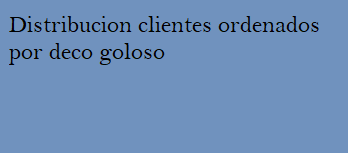
\includegraphics{DistribucionClientesDecoGoloso}
	\label{fig:DistribucionClientesDecoGoloso}
\end{figure}

\bigskip

Nuevamente, utlizando distintos sets de 200 $RandomKeys$ para cada instancia se generaron los siguientes resultados:

\begin{center}
\begin{tabular}{ |c|c|c|c|c|c|c|c|c|c| } 
\hline
$I$ & $\#N$ & $\#V$ & $tMax$ & $\#S$ & $B_{max}$ & $B_{min}$ & $B_{avg}$ & $i_{f}$ & $BTP_{max}$ \\
\hline
p2.2.k & 21 & 2 & 22.50 & 200 & 260 & 95 & 164 & 0.60 & 275   \\
p2.3.g & 21 & 3 & 10.70 & 200 & 140 & 95 & 122 & 0.84 & 145   \\
p3.4.p & 33 & 4 & 22.50 & 200 & 410 & 180 & 288 & 0.51 & 560   \\
p5.3.x & 66 & 3 & 40.00 & 200 & 525 & 305 & 412 & 0.26 & 1555   \\
p7.2.e & 102 & 2 & 50.00 & 200 & 163 & 31 & 96 & 0.33 & 290   \\
p7.4.t & 102 & 4 & 100.00 & 200 & 438 & 160 & 280 & 0.26 & 1077   \\
\hline
\end{tabular}
\end{center}

Todos los resultados promedio, mínimo y máximos mejoran considerablemente. Tal es así, que el $i_{f}$ en algunos casos es mayor al doble de lo obtenido en el decodificador simple. Por otro lado, se vuelve a observar la correlación entre tamaño de la instancia y el $i_{f}$.

\section{BRKGA}

En una primera intancia se implementa un BRKGA estandar. Dado una instancia de un problema, primero se genera la población inicial. Luego mientras no se cumpla la condición de parada, evolucionamos la poblacion. Es decir generamos una nueva generacion de soluciones a partir de la generación anterior como se explico en la sección BRKGA ~(ver sección~\ref{sec:brkga}).

\bigskip

Pseudocódigo de una vista macro general del algoritmo BRKGA implementado.

\bigskip

\begin{minipage}{\textwidth}
\begin{lstlisting} 
public Solution RunBrkga(ProblemManager problemManager)
{
    ProblemManager.InitializePopulation();

    while (!ProblemManager.StoppingRuleFulfilled())
        ProblemManager.EvolvePopulation();

    return ProblemManager.Population.GetMostProfitableSolution();
}
\end{lstlisting}
\end{minipage}

\bigskip

El objeto ProblemManager es el orquestrador del mi BRKGA, se setea con un objeto Configuración y el objeto PopulationGenerator. Tiene acceso de forma indirecta, atravéz de PopulationGenerator, de toda la información del problema (vehículos, clientes, tmax, etc.).

\subsection{Configuración}

A modo de poder testear distintas configuraciones del BRKGA, se creo un objeto $Configuration$ que setea todas las configuraciones que impactan en el resultado final del BRKGA. Este objeto es esencial para tunear el implementacion de una forma rápida y ordenada. Al centralizar todas las variables que podrían impactar en resultado final, ganaba mucho tiempo en al testear variaciones de mi implementación. Además, al estar centralizada toda la información variable se obtiene una lectura veloz del BRKGA que se esta usando. En otras palabras incrementamos nuestra capacidad de monitoreo y control de mi implementación.

\bigskip

\begin{minipage}{\textwidth}
\begin{lstlisting}
public class BrkgaConfiguration
{
	public string Description { get; }
	public int MinIterations { get; set; }
	public int MinNoChanges { get; set; }
	public int PopulationSize { get; set; }
	public decimal ElitePercentage { get; set; }
	public decimal MutantPercentage { get; set; }
	public int EliteGenChance { get; set; }
	public List<ILocalSearchHeuristic> Heuristics { get; set; }
	public int ApplyHeuristicsToTop { get; set; }
	public DecoderEnum DecoderType { get; set; }
	
	private void SetDescription();
}
\end{lstlisting}
\end{minipage}

\bigskip

\subsection{Descripción y codificación de las propiedades del objeto configuración}\label{sec:descrCongif}
Descripción de las propiedades del objeto Configuración:

\begin{itemize}
  \item \textbf{Description}: Es una especie de hash descriptivo de la instancia del objeto. Su funcionalidad es poder identificar rápidamente la configuración global del BRKGA. Solo puede ser seteado con el metodo SetDescription() que utilza la clave y el valor de el resto de las propiedades.
  \item \textbf{MinIterations}: Clave \textbf{MI}. Valor entero utilizado en la función de corte. Cantidad mínima de generaciones que debe genererar el BRKGA para finalizar. 
  \item \textbf{MinNoChanges}: Clave \textbf{MNC}. Valor entero utilizado en la función de corte. Cantidad de generaciones sin modificaciones del mejor beneficio necesario para cortar el algoritmo BRKGA.
  \item \textbf{PopulationSize}: Clave \textbf{PS}. Valor entero denota el tamaño de la población.
  \item \textbf{ElitePercentage}: Clave \textbf{EP}. Valor decimal en el itervalo $(0, 1)$ que determina el tamaño de la poblacion elite. 
  \item \textbf{MutantPercentage}: Clave \textbf{MP}. Valor decimal en el itervalo $(0, 1)$ que determina el tamaño mínimo de la poblacion mutante. 
  \item \textbf{EliteGenChance}: Clave \textbf{EGC}. Valor entero en el intervalo $(0, 100)$ que determina la probabilidad que tiene un key del padre elite, en transmitirse a su descendiente. 
  \item \textbf{Heuristics}: Clave \textbf{HEU}. Secuencia de heuristicas de busqueda local que se le aplicaran a la mejor solución de cada generación, a la cual no se le hayan aplicado las heuristicas locales aún. Se implementaron cuatro heuristicas locales:
	\begin{itemize}
		\item \textbf{Swap}: Valor \textbf{S}.
		\item \textbf{Insert}: Valor \textbf{I}.
		\item \textbf{2-Opt}: Valor \textbf{O}.
		\item \textbf{Replace}: Valor \textbf{R}.
	\end{itemize}  
  \item \textbf{ApplyHeuristicsToTop}: Clave \textbf{TOP}. Valor entero que denota la cantidad de soluciones a las cuales se les aplicaran las heuristicas de busqueda local.
  \item \textbf{DecoderType}: Clave \textbf{D}. Es una enumeracion que determina el decoder que se va a utilizar.
	\begin{itemize}
		\item \textbf{Simple}: Valor \textbf{S}.
		\item \textbf{Goloso}: Valor \textbf{G}.
	\end{itemize}  
\end{itemize}

\bigskip

El método SetDescription() toma las tuplas de clave y valor de todas las propiedades del objeto configuration excepto Description y genera un string intercalando con un separador.

\begin{minipage}{\textwidth}
\begin{lstlisting} 
public void SetDescription()
{ 
	var prop = Properties.Where(x => x.Name != "Description");
	var claveValores = prop.Select(p => p.Clave + "." + p.Valor);
	Description = string.Join(";", claveValores);
}
\end{lstlisting}
\end{minipage}


\begin{minipage}{\textwidth}
Luego dado un description podemos ver como esta configurado el BRKGA.

Ej: "MI.200;MNC.10;PZ.100;EP.0,3;MP.0,1;EGC.70;HEU.ISIRT;TOP.2;D.G"

\begin{itemize}
  \item MinIterations: 200
  \item MinNoChanges: 10
  \item PopulationSize: 100
  \item ElitePercentage: 0,3
  \item MutantPercentage: 0,1
  \item EliteGenChance: 70
  \item Heuristics: ISIRT. Que es la Secuencia Insert, Swap, Insert, Replace, 2-Opt.
  \item ApplyHeuristicsToTop: 2
  \item DecoderType: Decodificador Goloso
\end{itemize}
\end{minipage}

\subsection{Inicialización de la Población}

Utilizando $PopulationSize$ del objeto $Configuration$ seteo el tamaña de la población. Luego para generar la población inicial se genereran $PopulationSize$ vectores de enteros aleatorios de tamaño $\#clientes$ de la instancia del problema. Este conjunto de vectores se lo pasa como argumento al decodificador, quien genere un individuo por cada vector de enteros aleatorios.

\subsection{Condición de parada}

En un principio la condición de parada era simple, el bucle terminaba cuando iteraba una $x$ cantidad de veces seteado en el objeto $Configurations$ por $MinIerations$. Es decir que el bucle principal cortaba luego de evolucionar la poblacion $MinIerations$ veces. Luego de analizar las últimas generaciones de la solución y ver que era frecuente que la mejor solución se habia generado recientemente, agregue una condicion de corte adicional. Ahora, para cortar ademas de la condición anterior, el beneficio de la mejor solución no debería haberse modificado durante las últimas $n$ generaciones . Es decir durante las últimas $n$ genereciones no debe haber aparecido una nueva mejor solución. Este valor es ajustable desde la propiedad $MinNoChanges$ del objeto $Configurations$.

\bigskip

\begin{minipage}{\textwidth}
\begin{lstlisting} 
public bool StoppingRuleFulfilled()
{ 
    return GenerationNum >= MinIterations && NoChanges();
}
private bool NoChanges()
{
	var currentProfit = CurrentBestSolution.GetProfit();
	return LastProfits.All(p => p == currentProfit);
}
\end{lstlisting}
\end{minipage}

\subsection{Evolución de la población}

Se toma la población y se los ordena descendientemente segun su beneficio calculado por la función objetivo. Se setea la población de elite y la non-elite. La población de elite son los mejores $x$ individuos de la población. Siendo $x$ un porcentaje de la población total seteado con la propiedad $ElitePercentage$ del objeto $Configuration$. La población non-elite son todos aquellos individuos no incluídos en la población de elite. Luego se generan $y$ individuos mutantes, $y$ es un porcentaje de la población total seteado por la propiedad $MutantPercentage$. Pasan a la nueva genereción todos los individuos de la población de elite y se agregan los de la población mutante. Finalmente se completa la nueva generación emparentando individuos de la población de elite con individuos de la población non-elite. Los padres son elegidos al azar y el proceso de apareamiento se realiza como se describe en el la sección BRKGA ~(ver sección~\ref{sec:brkga}). Durante el apareamiento, no es tan extraño que se genere una solución identica a otra ya existente en la población. De modo de no repetir soluciones, antes de insertar el individuo resultante se verifica que no exista otra solución idéntica en la nueva generación.

\bigskip

\begin{minipage}{\textwidth}
\begin{lstlisting}
public Population Evolve(Population population)
{
    var ordPopulation = population.GetOrderByMostProfitable();
    var elites = ordPopulation.Take(EliteSize);
    var nonElites = ordPopulation.Skip(EliteSize).Take(NonEliteSize);
    var mutatants = Generate(MutatansSize);
    var evolvedPopulation = new pop(elites, mutatants);
    while (evolvedPopulation.Size() < PopulationSize)
    {
		var anElite = GetRandomItem(elites);
		var aNoneElite = GetRandomItem(nonElites);
        var childSolution = Mate(anElite, aNoneElite);
        if (evolvedPopulation.Any(x => x.Equals(childSolution)))
            evolvedPopulation.Add(GenerateSolution());
        else
            evolvedPopulation.Add(childSolution);
    }
    return evolvedPopulation;
}
\end{lstlisting}
\end{minipage}

\begin{minipage}{\textwidth}
\begin{lstlisting}
private Solution Mate(Solution eliteP, Solution nonEliteP)
{
	var childRandomKeys = new List<RandomKey>();
	for (var index = 0; index < eliteP.RandomKeys.Count; index ++)
	{
		int key = 0;
		if(Random.Next(100) >= EliteGenChance)
			key = eliteP.RandomKeys[index].Key;
		else
			key = nonEliteP.RandomKeys[index].Key;
		var randomKey = new RandomKey(key, index);
		childRandomKeys.Add(randomKey);
	}
	return Decoder.Decode(childRandomKeys, ProblemInfo);
}
\end{lstlisting}
\end{minipage}

\bigskip

Como mencioné anteriormente, los individuos mutantes son individuos generedos a partir de un vector de RandomKeys, del mismo modo que la población inicial. Con el fín de mostrar lo simple que es la generación de un nuevo vector de RandomKeys, presento el pseudocodigo del GenerateSolution que al final termina llamando al método decode del decoder descripto anteriormente.

\bigskip

\begin{minipage}{\textwidth}
\begin{lstlisting}
private Solution GenerateSolution()()
{
	var randomKeys = new List<RandomKey>();
	for(i = 0; i < ProblemInfo.Clients.Length; i++)
	{
		var key = Random.Next(1000);
		var randomKey = new RandomKey(key, index);
		randomKeys.Add(randomKey)
	}
	return Decoder.Decode(randomKeys, ProblemInfo);
}
\end{lstlisting}
\end{minipage}

\bigskip

Verificar que dos soluciones son iguales tiene un costo muy bajo en BRKGA. Esto se debe a que el decodificador es un algoritmo deterministico. Por lo tanto para dos vectores de RandomKeys cuyo orden de clientes que genere sea el mismo, el decodificador generará la misma solución. Luego lo unico que hay que comparar es el hash de ambas soluciones y esto se puede hacer en $O(1)$. El hash de una solución, se calcula una sola vez cuando se construye la solución a partir de su vector de RandomKey. El hash es una concatenación de la propiedad PositionIndex de cada RandomKey en el vector ordenados por la propiedad Key, itercalados con un separador. Es decir, es el orden de la cuidades que toma el decoder intercalados con un separador. Si ya existe un individuo con el mismo hash, se genera una solución mutante y continua el apareamiento de otros dos individuos. Decidí no reintentar el apareamiento entre los dos padres que genereron la solución ya existente, porque consideré que la probabilidad de volver a generar nuevamente una solución existente es alta. Ademas, aún si en un segundo intento no generera una solución idéntica a alguna de la nueva población, lo más seguro que la solución originada se muy cercana a una existente. Luego tome esta desición para optimizar el apareamiento y disminuir soluciones dentro de un mismo vecindario por genereración.

\bigskip

\begin{minipage}{\textwidth}
\begin{lstlisting}
private string pseudoHash;
public string GetHash()
{
	if (!string.IsNullOrEmpty(pseudoHash))
		return pseudoHash;
		
	var ork = RandomKeys.OrderBy(r => r.Key)
	pseudoHash = string.Join("@", ork.Select(k => k.PositionIndex));
	return pseudoHash;
}
\end{lstlisting}
\end{minipage}

\bigskip

En una primera instancia se insertaban los individuos sin verificar que la solución no existiese en la población. Dado una población de soluciones no repetidas, la probabilidad de de generar una solucion existente al evolucionar la población, es baja. Aún así, una vez que sucede, la probabilidad de generar otra más aumenta considerablemente ya que ahora hay mas probabilidades de utilizar padres ídenticos. Si además la solución repetida se ecuentra dentro del subconjunto de elite, la probabilidad aumenta aún más. Esto generaba un efecto bola de nieve donde cada nueva generación tenía cada vez más individuos repetidos. Incluso se llego al caso donde toda una población constituía de una unica solución excepto por las soluciones mutantes. Esto reducía ampliamente la cantidad de soluciones diferentes exploradas, luego reducía fuertemente la frecuencia con la que una nueva mejor solución aparecía. Además si uno tiene varios individuos iguales en una solución, el algoritmo se vuelve menos eficiente ya que repite trabajo en donde obtiene los mismos resultados. Entonces el costo total de validar unicidad en la inserción, que conlleva un orden de complejidad $O(PopulationSize * NonElitePopulationSize)$, resulta muy bajo comparado con el costo de trabajar con multiples soluciones repetidas.

\subsection{Resultados de la primer versión}

La primer versión del BRKGA para TOP no incluía el objeto de configuración y permitía insertar soluciones repetidas en una misma generación. Los indices de efectividad que mostrare a continuación corresponden con una primera versión que no admitía repetidos y el objeto configuracion. Para estos primeros resultados genere resultados por intancia y utilice una configuración estandar sin heurisitcas locales aún:\\ 'MI.250;MNC.10;PS.100;EP.0,3;MP.0,1;EGC.70;HEU.;TOP.0;MI.G' (ver sección~\ref{sec:descrCongif}).

\bigskip

\begin{center}
\begin{tabular}{ |c|c|c|c|c|c|c|c|c|c| } 
 \hline
$I$ & $\#N$ & $\#V$ & $tMax$ & $T_{avg}$ & $B_{max}$ & $B_{min}$ & $B_{avg}$ & $i_{f}$ & $BTP_{max}$ \\
\hline
p2.2.k & 21 & 2 & 22.50 & 2977 & 260 & 240 & 249 & 0.91 & 275  \\
p2.3.g & 21 & 3 & 10.70 & 1990 & 145 & 145 & 145 & 1.00 & 145  \\
p3.4.p & 33 & 4 & 22.50 & 6482 & 450 & 430 & 438 & 0.78 & 560  \\
p5.3.x & 66 & 3 & 40.00 & 17908 & 660 & 610 & 635 & 0.41 & 1555  \\
p7.2.e & 102 & 2 & 50.00 & 8753 & 246 & 204 & 217 & 0.75 & 290  \\
p7.4.t & 102 & 4 & 100.00 & 31532 & 513 & 458 & 481 & 0.45 & 1077  \\
\hline
\end{tabular}
\end{center}

\bigskip

De estos primeros resultados podemos ver que el BRKGA puro sin otras heuristicas funciona muy bien para instancias de testeo pequeñas esta versión funcionaba tan bien como Chao, Golden y Wasil (CGW), Tang y Miller-Hooks (TMH) y Archetti, Hertz, Speranza (AHS). Esto se refleja en la instancia \textit{p2.3.k} que siempre se llegó a la mejor solución posible y en \textit{p2.2.k} donde el $i_f$ supera el 0.90. Luego a medida que incrementa el tamaño de la instancia, disminuye el $i_f$. Una observació que quiero destacar de estos resultados es sobre el $i_f$ de la instancia 'p7.2.e'. Notar que tiene tantos nodos como 'p7.4.t' y sin embargo su $i_f$ ampliamente mayor. Esto se puede estar dando por que solo son 2 vehículos, en vez de 4, adicionalmente la distancia máxima, $tMax$, es 50 en vés de 100 reduciendo la combinatoria de soluciones posibles.


\bigskip

Como estos resultados no eran satisfactorios, tomé las dos intancias de este subconjunto con menor $i_{f}$ y las utilice para testear distintas configuracions. Probé multipes variaciones del objeto configuración. A continuación el resultado de algunas de tales variaciones:

\bigskip


\begin{center}
\begin{tabular}{ |c|c|c|c|c|c|c|c|c|c|c|c| } 
 \hline
$I$ & $\#N$ & $\#V$ & $tMax$ & $C$ & $\#S$ & $T_{avg}$ & $B_{max}$ & $B_{min}$ & $B_{avg}$ & $i_{f}$ & $BTP_{max}$ \\
\hline
p5.3.x & 66 & 3 & 40.00 & 1 & 10 & 60782 & 700 & 635 & 656 & 0.42 & 1555  \\
p5.3.x & 66 & 3 & 40.00 & 2 & 10 & 23363 & 660 & 620 & 636 & 0.41 & 1555  \\
p5.3.x & 66 & 3 & 40.00 & 3 & 10 & 22357 & 685 & 615 & 643 & 0.41 & 1555  \\
p5.3.x & 66 & 3 & 40.00 & 4 & 10 & 7311 & 555 & 475 & 498 & 0.32 & 1555  \\
p5.3.x & 66 & 3 & 40.00 & 5 & 10 & 54239 & 750 & 630 & 668 & 0.43 & 1555  \\
p7.4.t & 102 & 4 & 100.00 & 1 & 10 & 143760 & 542 & 472 & 506 & 0.47 & 1077  \\
p7.4.t & 102 & 4 & 100.00 & 2 & 10 & 42255 & 504 & 471 & 485 & 0.45 & 1077  \\
p7.4.t & 102 & 4 & 100.00 & 3 & 10 & 45952 & 542 & 463 & 488 & 0.45 & 1077  \\
p7.4.t & 102 & 4 & 100.00 & 4 & 10 & 11587 & 322 & 268 & 284 & 0.26 & 1077  \\
p7.4.t & 102 & 4 & 100.00 & 5 & 10 & 96642 & 509 & 478 & 491 & 0.46 & 1077  \\
\hline
\end{tabular}
\end{center}

\bigskip

Configuraciones: 
\begin{itemize}
  \item \textbf{C = 1}: MI.100;MNC.100;PS.500;EP.0,30;MP.0,05;EGC.70;HEU.;TOP.0;D.G
  \item \textbf{C = 2}: MI.150;MNC.30;PS.200;EP.0,25;MP.0,05;EGC.60;HEU.;TOP.0;D.G 
  \item \textbf{C = 3}: MI.150;MNC.70;PS.200;EP.0,30;MP.0,10;EGC.70;HEU.;TOP.0;D.G
  \item \textbf{C = 4}: MI.150;MNC.70;PS.200;EP.0,30;MP.0,10;EGC.70;HEU.;TOP.0;D.S
  \item \textbf{C = 5}: MI.250;MNC.50;PS.250;EP.0,15;MP.0,05;EGC.50;HEU.;TOP.0;D.G 
\end{itemize}

\bigskip

Como sintesis de estos resultados digo que la configuracion basica poco influye en el beneficio final de la solución. En el caso de la instancia 'p5.3.x', el $i_{f}$ siempre se encuentra en el intervalo [0.41,0.43] y en en 'p7.4.t' el intervalo es [0.45,0.47]. Para ambas intancias hay una configuración que es claramente peor y es la configuracion \textbf{C = 4} donde se utiliza el decodificar \textbf{simple} en vez del \textbf{goloso}. Luego claramente en esta version del BRKGA el decodificador tiene gran impacto en resultado final. Lamentablemente el resto de las configuraciones impacta muy poco en el beneficio total cuando la instancia del problema es grande (Minima cantidad de iteraciones, minima cantidad de iteraciones sin cambios, tamaño de la poblacion, poblacion elite, etc). Si impactan en el tiempo en que finaliza el algoritmo. Cuando llegue a este punto en mi trabajo, considere que tenía dos opciones por donde continuar. La primera, crear nuevos decodificadores. La segunda, agregar heuristicas de busqueda local para aplicar a las mejores individuos de cada generación. Tome el camino de la segunda opción.

\bigskip

\section{Heuristicas de busqueda local}

En pos de optimizar los resultados mencionados anteriormente se implementaron heuristicas de busqueda local. La idea fue aplicar estas heurísticas a la mejores $x$ soluciónes de cada nueva generación. Donde $x$ toma el valor de la propiedad $ApplyHeuristicsToTop$. En caso de que a la solución ya se le hubiese aplicado las heuristicas en una generación anterior, se aplican a la siguiente mejor solución. Esto puede suceder ya que las mejores soluciones pertenecen al conjunto de elite, y todos los indiviuos del conjunto de elite pasan a la siguiente generación. La idea de implementar heuristicas de busqueda local la obtuve de la publicación \textit{A guided local search metaheuristic for the team orienteering problem.} de Vansteenwegen et al. \cite{VansteenwegenSouffriauBergheOudheusden}. Todas las heuristicas de busqueda local al modificar una solucion, la misma sigue siendo una solucion valida. Es decir se siguen respetando las restricciones de distancia y la cantidad de vehiculos. 

\subsection{Center of Gravity}

Para las heuriticas de busqueda local Insert y Replace se deben tomar una lista de clientes a considerar con algun orden. Este orden es importante ya que queremos empezar por las mejores opciones. El orden de clientes que se utiliza es por su distancia al centro de gravedad (COG) de una ruta. A menor distancia, mayor prioridad tendra el cliente. Implementé el calculo de COG de la forma que lo describen Vansteenwegen et al. \cite{VansteenwegenSouffriauBergheOudheusden}. La coordena COG de una ruta se calcula con las siguietes formulas:

\begin{equation}
x_{cog} = (\sum_{\forall i \in ruta} x_i * B_i) / \sum_{\forall i \in ruta} B_i
\end{equation}

\begin{equation}
y_{cog} = (\sum_{\forall i \in ruta} y_i * B_i) / \sum_{\forall i \in ruta} B_i
\end{equation}

\bigskip

Donde $x_i$ e $y_i$ son las coordenadas de un cliente de la ruta y $B_i$ es su beneficio.
El calculo de COG tiene una complejidad de $O(ruta.Length)$. No es tan costoso, de todos modos como no quiero realizar calculos innecesarios, el COG de una ruta solo se calcula cuando se necesita, es decir cuando se es. Ademas se calcula una vez y se mantiene en memoria. Cuando se modifica la ruta, actualizo el COG.

\bigskip

Sea $r$ una ruta:

\begin{equation}
r.x_{cog} =  \frac{\sum_{\forall i \in ruta} x_i * B_i}{\sum_{\forall i \in ruta} B_i}  = \frac{r.x_{cog.num}}{r.x_{cog.den}}
\end{equation}

\bigskip

Sea $r' = r.Remove(c_j)$ con $c_j$ cliente y $c_j \in r$:

\begin{equation}
r'.x_{cog} =  \frac{\sum_{\forall i \in ruta \wedge i \neq j} x_i * B_i}{\sum_{\forall i \in ruta \wedge i \neq j} B_i}  = \frac{r.x_{cog.num}-x_j*B_j}{r.x_{cog.den}-B_j}
\end{equation}

\bigskip

Sea $r'' = r.Add(c_k)$ con $c_k$ cliente y $c_k \notin r$:

\begin{equation}
r'.x_{cog} =  \frac{(\sum_{\forall i \in ruta} x_i * B_i) + x_k * B_k}{(\sum_{\forall i \in ruta} B_i) + B_k}  = \frac{r.x_{cog.num}+x_k*B_k}{r.x_{cog.den}+B_k}
\end{equation}

\bigskip

Luego actualizar el COG de una ruta al agregar ó remover un cliente tiene una complejidad de $O(1)$ si guardamos en memoria y actualizamos los valores de $x_{cog.num}$ y $x_{cog.den}$ para cada ruta (Lo mismo aplica para la coordenada $y$).

\bigskip



\subsection{Swap}

El objetivo de esta heuristica es encontrar e intercambiar clientes entre dos rutas distintas con el fin de disminuir la suma de las distancias recorridas de ambas rutas mientras sigan respetando la restricción de distancia máxima por vehículo. Es decir dados $v_a$, $v_b$ vehiculos y sus respectivas rutas $r_a$, $r_b$, se puede realizar un swap entre sus rutas si existe un cliente $c_{a_i}$ en la ruta de $r_a$ y otro cliente $c_{b_j}$ en $r_b$ tal que agregando $c_{a_i}$ en alguna posición de $r_b$ y agregando $c_{b_j}$ en alguna posición de $r_a$, valen:

\begin{equation*}
r_a.Dist + r_b.Dist < r_a'.Dist + r_b'.Dist \nonumber
\end{equation*}

\begin{equation*}
r_a'.Dist \leq v'_a.dMax
\end{equation*}

\begin{equation*}
r_b'.Dist \leq v'_b.dMax
\end{equation*}

Al aplicar esta heuristica a una solución, para todos par de rutas se ejecuta el método \textit{SwapDestinationsBetween}. Si hay $n$ rutas, la cantidad de pares de rutas es $n * (n-1) / 2$. \textit{SwapDestinationsBetween} prueba cada cliente de la ruta $a$ con cada cliente de la ruta $b$, si efectivamente conviene hacer un swap, lo realiza y continua probando pares de clientes. De modo de no estar cambiando multiples veces un mismo cliente entre dos rutas en una misma ejecución de \textit{SwapDestinationsBetween}, cuando se cambia de ruta a un cliente, se lo banea de cambios hasta que no termine la actual ejecución de \textit{SwapDestinationsBetween}. La metaheuristica Swap no mejora el beneficio total de una solución. Lo que hace es disminuir la distancia recorrida de alguna ruta, lo que aumente la probabilidad de encontrar algun cliente no visitado que se pueda insertar en alguna de las rutas modificadas.

\bigskip

\begin{minipage}{\textwidth}
\begin{lstlisting}
// Dentro de clase SwapHeuristic
public void ApplyHeuristic(Solution solution)
{
	var changed = false;
	var combinations = GetCombinationsFor(solution.Vehicles.Count);
	foreach (var combination in combinations)
	{
		var v1 = solution.Vehicles[combination.Left];
		var v2 = solution.Vehicles[combination.Right];
		changed = changed || SwapDestinationsBetween(v1, v2);
	}
	if(changed)
		solution = Encoder.UpdateRandomKeys(solution);
}
\end{lstlisting}
\end{minipage}

\begin{minipage}{\textwidth}
\begin{lstlisting}
public bool SwapDestinationsBetween(Vehicle v1, Vehicle v2)
{
	var changed = false;
	var v1Bans = new Dictionary<int, bool>();
	var v2Bans = new Dictionary<int, bool>();
	for (var i = 0; i < v1.Route.RouteLenght(); i++)
	{
		if(v1Bans.ContainsKey(i)) 
			continue;
		for (var j = 0; j < v2.Route.RouteLenght(); j++)
		{
			if (v2Bans.ContainsKey(j)) 
				continue;
			if (!Swaps(i, j, ref leftRoute, ref rightRoute)) 
				continue;
			changed = true;
			v1Bans.Add(i, true);
			v2Bans.Add(j, true);
			break; // Para que cambie i
		}
	}
	return changed;
}
\end{lstlisting}
\end{minipage}

\bigskip

El orden de complejidad del método ApplyHeuristic de la clase SwapHeuristic es:

\begin{equation*}
O((n * (n-1) / 2 ) * clientes/n * clientes/n) \approx O(clientes^2/2)
\end{equation*}

\subsection{Insert}

El objetivo de esta heuristica es encontrar una posición en alguna ruta para un cliente no visitado. Básicamente para cada vehiculo y cada cliente no visitado se busca en que posición se puede insertar minimizando el incremento de distancia. Si la distancia resultante es menor a la distancia máxima del vehiculo, se inserta el cliente en tal posicion. El orden en que se toman los clientes no visitados es segun su distancia al COG de la ruta a optimizar, de forma ascendente.

\begin{minipage}{\textwidth}
\begin{lstlisting}
// Dentro de clase InsertHeuristic
public void ApplyHeuristic(Solution solution)
{
	// Lista de los clientes no visitados
	var changed = false;	
	var uClients = solution.GetUnvistedClients;	
	var vehicles = solution.Vehicles;
	foreach (var vehicle in vehicles)
	{
		vehicle.Route.ActivateCog();
		uClients = uClients.OrderBy(x => vehicle.DistanceToCog(x));	
		for (var index = 0; index < uClients.Count; index++)
		{
			var res = AnalizeInsert(solution, vehicle, uClients[index]);
			if (res.CanBeInserted)
			{
				vehicle.AddDestinationAt(uClients[index], res.BestPosition);
				uClients.Remove(uClients[index]);
				changed = true;
			}
		}
	}
	if(changed)
		solution = Encoder.UpdateRandomKeys(solution);
}
\end{lstlisting}
\end{minipage}

\bigskip

Como menciones en sobre la implementacion de COG, solo se utiliza cuando es necesario. Luego para cada vehiculo lo primero que hace es activar el COG. Segundo, por cada cliente no visitado hasta el momento se analiza el insert. El método \textit{AnalizeInsert} retorna un objeto que tiene seteado dos campos importantes. Un campo bool que denota que el cliente puede ser insertado o no en el vehiculo consultado. Y otro campo que tiene la posicion donde se debe insertar, en caso de poder insertarlo. En caso de poder insertar el cliente, este se lo agrega al vehiculo que actualiza su COG, y se remueve el cliente de la lista de no visitados. El orden de complejidad del método ApplyHeuristic de la clase InsertHeuristic es: 

\begin{equation*}
0(vehiculos * clientesNoVisitados * mediaClientesEnRuta)
\end{equation*}

\subsection{2-opt}

El algoritmo 2-opt es un simple algoritmo de búsqueda local propuesto por Croes \cite{Croes}. El fin es buscar un orden alternativo de los clientes visitados en una dentro de una misma ruta, de modo que disminuya la distancia recorrida de la misma. Es decir, un swap de posiciones de dos clientes dentro de una misma ruta.

\begin{minipage}{\textwidth}
\begin{lstlisting}
// Dentro de clase 2-opt
public void ApplyHeuristic(Solution solution)
{
	var index = 0;
	var changed = false;	
	var vehicles = solution.Vehicles;	
	while (index < vehicles.Count)
	{
		var currentDistance = vehicles[index].Route.GetDistance();
		changed = changed || Do2OptSwap(vehicles[index]);
		index++;
	}
	if(changed)
		solution = Encoder.UpdateRandomKeys(solution);
}
\end{lstlisting}
\end{minipage}

\begin{minipage}{\textwidth}
\begin{lstlisting}
private bool Do2OptSwap(Vehicle vehicle)
{
	var changed = false;	
	var combinations = GetCombinationsFor(vehicle.Route.GetDistance());
	var index = 0;
	while (index < combinations.Count)
	{
		var position1 = combinations[index].Item1 - 1;
		var position2 = combinations[index].Item2 - 1;
		var swaped = vehicle.Route.SwapIfImprovesDistance(position1, position2);
		if (!swaped)
			index++;
		changed = true;
		index = 0;
	}
	return changed;
}
\end{lstlisting}
\end{minipage}

\bigskip

Basicamente a cada vehículo le aplica el 2-opt. El método Do2OptSwap primero obtiene una lista de las permutaciones posibles. Luego por cada combinacion intenta hacer un swap dentro de la ruta. Si el swap sucede, luego vuelve a empezar desde el principio ya que ese cambio puede generar nuevos cambios. Como el swap solo sucede cuando la nueva distancia es estrictamente menor, el loop siempre termina. Una ruta no puede estar mejorando infinitamente. Este algoritmo tiene un order de complejidad $0(vehiculos * mediaClientesEnRuta  * (mediaClientesEnRuta - 1) / 2) ~ 0 (vehiculos * mediaClientesEnRuta^2 / 2)$.

\subsection{Replace}

Esta heuristica busca intercambiar un cliente no visitado por uno visitado de una ruta de modo que aumente el beneficio de la ruta. Del mismo modo que la heuristica insert, los clientes no visitados se toman en orden segun su distancia al COG de la ruta, empezndo por los mas cercanos.

\begin{minipage}{\textwidth}
\begin{lstlisting}
// Dentro de la clase ReplaceHeuristicas
public void ApplyHeuristic(Solution solution)
{	
	var vehicles = solution.Vehicles;
	var changed = false;	
	foreach (var vehicle in vehicles)
		changed = changed || Replace(solution, vehicle);
	if(changed)
		solution = Encoder.UpdateRandomKeys(solution);
}
\end{lstlisting}
\end{minipage}

\begin{minipage}{\textwidth}
\begin{lstlisting}
private bool Replace(Solution solution, Vehicle vehicle)
{
	var unvisited = solution.GetCurrentUnvistedDestination;
	var changed = false;
	vehicle.Route.ActivateCog();
	uClients = uClients.OrderBy(x => vehicle.DistanceToCog(x));	

	foreach (var client in uClients)
	{
		var res = AnalizeInsert(solution, vehicle, client);
		vehicle.AddDestinationAt(destination, res.BestInsertPosition);
		if (!res.CanBeInserted)
		{
			var removedClient = RemoveWorstOrDefault(vehicle, client);
			changed = changed || removedClient.Id != client.Id;
		}
		else
			changed = true;
	}
	return changed;
}
\end{lstlisting}
\end{minipage}

\bigskip

La heurística de replace es muy parecida al insert y esto se refleja en el pseudocódigo. Ante un cliente no visitado, lo primero que hace es analizar si se puede insertar y cual es la mejor posición donde se puede insertar, llamando al método \textit{AnalizeInsert}. Luego sin siquiera verificar si realmente se puede insertar, lo inserta en la posición que menos incrementa la distancia de la ruta. Este es el único momento de toda la implementación donde puede existir una solución invalida. Por lo tanto ahora se fija si realmente se podía insertar. En caso afirmativo, continua con el siguiente cliente. En caso contrario remueve de la ruta el peor destino, que en el peor de los casos es el mismo cliente que se acaba de insertar. Cualquier otro cliente que se remueva de la ruta significará que se efectuo un replace y aumento el beneficio total de la ruta. Replace tiene una complejidad de $O(vehiculos * clientesNoVisitados * mediaClientesEnRuta * 2)$. 

\subsection{Encoder}

Agregar heuristicas de busqueda local entre generación de poblaciones conlleva un problema que debe resolverse. Al mejorar la solución, se modifican sus rutas. Ahora bien, si no se modifica su genética, es decir su \textit{RandomKeys}, sus descendientes heredarán los genes que generan una solucion no optimizada por las búsquedas locales. Del mismo modo que una persona no hereda las cirujias esteticas de sus padres. 

\begin{equation*}
ApplyHeuristic(s) \neq Decoder.Decode(s.RandomKeys, ProblemInfo)
\end{equation*}

Para solucionar esto se debe modificar el vector aleatorio de enteros, \textit{RandomKeys}, de la solución mejorada de modo que al decodificar tal vector aleatorio de enteros, genere la solución modificada. Como mencioné en el sección del Decodificador (ver sección~\ref{sec:ordenDeco}), los clientes se ordenan de forma ascendente por la propiedad \textit{Key} del objecto \textit{RandomKey} asociado según la propiedad \textit{PositionIndex}. Luego el primer cliente con el que trabaja el decoder, es el cliente con menor \textit{Key} de su \textit{RandomKey} asociado. Algo que no menciones en Decoder es que el primer vehiculo por el que empieza es por el de menor \textit{Id} ya que los ordena por su \textit{Id} de forma ascendente. Los vehiculos son indistinguibles al tener el mismo \textit{tMax} en el benchmark de intances de problemas utilizado. De todos modos ahora debo respetar la desición que tome en el decoder. Por lo tanto tomo el primer cliente de la ruta del vehículo con menor \textit{Id} y a ese cliente le voy a asociar el {RandomKey} que tenga el menor key. Así, cuando el decoder inicie lo primero que hará es tomar este cliente e intentara adjudicarselo al primer vehículo que sera el de menor \textit{Id}. Luego tomaré el segundo cliente del mismo vehículo y le asignare el segundo \textit{RandomKey} de menor \textit{Key}. Y así sucesivamente, hasta tener mapeados todos los clientes del primer vehículo con su nuevo \textit{RandomKey}. Luego repito el procedimiento con los clientes del siguiente vehículo ordenados por \textit{Id} ascendentemente. Finalmente, no tendré mas vehículos y quedará un resto de clientes no visitados a los cuales le tengo que asociar algún \textit{RandomKey}. A estos clientes podría asignarle cualquier RandomKey. Aún así, en pos de disminuir los cambios genéticos sobre el individuo, les asigne un \textit{RandomKey} tal que entre ellos mantuvieran el mismo orden que mantenian antes de la optimización. Es decir, dentro de los clientes no visitados, el cliente que previamente tenia el \textit{RandomKey} con menor \textit{Key}, le asigne el \textit{RandomKey} de menor \textit{Key} que habia disponible. Con esto me aseguro que todos los clientes que estaban en el primer vehículo, esten en el primer vehiculo al decodificar el random keys. Este proceso puede verse en la figura \ref{fig:codificacionDeSolucion}.

\bigskip

\begin{figure}[h]
	\caption{Como se codifica una solución}
	\centering
	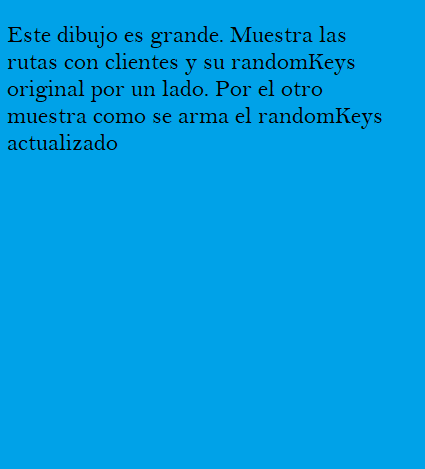
\includegraphics{codificacionDeSolucion}
	\label{fig:codificacionDeSolucion}
\end{figure}

\bigskip

Ahora bien, digamos que existe un escenario donde el decoder se encuentra trabajando con un RandomKeys que fue generado por el encoder y sucede lo siguiente. Al agregar al último cliente de la primer ruta, como es un decoder goloso, intentará agregar a la primer ruta al resto de los clientes y supongamos que efectivamente encuentra uno. Cuando vi la posibilidad de este escenario, decidi agregar unos delimitadores de modo que si el decoder se encuentra con uno, siempre cambie de vehículo. Estos delimitadores son modelas por la propiedad, \textit{ForceVehicleChangeAfterThis}, con la que extendia al objeto \textit{RandomKey}. De este modo el Decoder, luego de utilizar el \textit{RandomKey}, se fija si \textit{ForceVehicleChangeAfterThis} es \textit{true} y si lo es, deja de intentar agregar clientes a la ruta del vehículo actual, pasando al siguiente. Los delimitadores no son heredados a los descendientes. Estos delimitadores me aseguran que valga: 

\begin{equation} \label{eq:1}
ApplyHeuristic(s) = Decoder.Decode(s.RandomKeys, ProblemInfo)
\end{equation}

\bigskip

En caso de no tener los delimitadores, como dije antes, una ruta podría tener un cliente extra, que para fines del algoritmo, no es malo. Al agregar un cliente, hay dos opciones. La primera es que el cliente perteneciera al subconjunto de clientes que no estaba visitado. En este caso aumentaria el beneficio total. Pero para que esto suceda, la heuristica de insert no debería haber funcionado correctamente ó no fue la última en aplicarse. En caso de que el cliente perteneciece a otro vehículo, el beneficio total no se modifica. El peor escenario es que este segundo vehiculo se quede con el cliente de un tercer vehiculo, sucediendo un especie de cambios en cadenados de clientes entre una secuencia de vehículos sin decrementar el beneficio total. Luego por mas que tomé la desicion de agregar los delimitadores, considero que ambas opciones eran igual de buenas considerando solamente la función objetivo. Como agregar los delimitadores asegura la valides de la ecuación \ref{eq:1}.

%\begin{minipage}{\textwidth}
\begin{lstlisting}
public static Solution UpdateRandomKeys(Solution s);
{
	var randomKeys = s.GetOrderedRandomKeys();
	// Todas las keys ordenadas ascendente
	var keys = randomKeys.Select(k => k.Key).ToList();
	var positionIndexes = new List<int>();
	// Get Position Indexes from Visited Clients
	foreach (var r in s.Routes)
	{
		var d = r.GetDestinations();
		var rpi = d.Select(d => d.PositionIndex);
		positionIndexes.AddRange(rpi);
	}
	// Get Position Indexes from Unvisited Clients
	var uPositionIndexes = GetUnvisitedPositionIndexes(randomKeys, newRoutes);
	positionIndexes.AddRange(unvistedPositionIndexes);

	// Hay un break por cada cantidad de clientes en ruta 
	var breaks = new Queue(newRoutes.Select(r => r.GetDestinations.Count));

	var newRandomKeys = new List<RandomKey>();
	var endRoute = false;
	var acumBreak = 0;
	for (var index = 0; index < keys.Count; index++)
	{
		if (breaks.Count > 0)
		{		
			endRoute = index + 1 == (int)breaks.Peek() + acumBreak;
			if (endRoute)
				acumBreak += (int)breaks.Dequeue();
		}		
		var randomKey = new RandomKey()
		{
			Key = keys[index],
			PositionIndex = positionIndexes[index],
			ForceVehicleChangeAfterThis = endRoute
		};
		newRandomKeys.Add(randomKey);
	}
	s.SetRandomKeys(newRandomKeys);
	return s;
}
\end{lstlisting}
%\end{minipage}

\subsection{Secuencia de Aplicación de las Heuristicas}

Todas las heuristicas mencionadas, implementan el interfaz:

\begin{lstlisting}
public interface ILocalSearchHeuristic
{
	void ApplyHeuristic(Solution solution);
}
\end{lstlisting}

Esto lo hice así de modo de poder inicializar el vector de heuristicas a aplicar en la creación del algoritmo BRKGA. Luego al momento de aplicar las búsquedas locales, llama en orden de inserción de tal vector y ejecuta su metodo ApplyHeuristic. Así se pueden testear multiples ordenes distintos de búsquedas locales con un simple modificación del parametro de entrada del constructor del BRKGA. El orden en que las heuristicas se aplican es muy relevante. Por ejemplo, si la última heuristica que aplicamos es Swap o 2-Opt, luego la distancias disminuídas de las rutas no sería aprobechado por ninguna cliente.

\bigskip

Configuraciones: 
\begin{itemize}
  \item \textbf{Comun a todas}: MI.200;MNC.50;PS.150;EP.0,3;MP.0,1;EGC.70;TOP.2
  \item \textbf{C = 1}: HEU.IROS;D.G
  \item \textbf{C = 2}: HEU.SIORSOR;D.G
  \item \textbf{C = 3}: HEU.SIORSOR;D.S
  \item \textbf{C = 4}: HEU.SOIR;D.G
  \item \textbf{C = 5}: HEU.SOIR;D.S
  \item \textbf{C = 6}: HEU.SOISOIR;D.G
\end{itemize}

Recordando los codigos de HUE: 
\begin{itemize}
  \item \textbf{I}: Insert (Cliente no visitado)
  \item \textbf{R}: Replace (Cliente no visitado por uno visitado)
  \item \textbf{0}: 2-Opt (Swap dentro de una misma ruta)
  \item \textbf{S}: Swap (Swap entre dos rutas distintas)
\end{itemize}

\bigskip

Genere soluciones para las mismas seis instancias diversas, varian en la configuración solamente el orden de las búsquedas locales y el decodificador obteniendo los siguientes resultados:

\bigskip

\begin{center}
\begin{tabular}{ |c|c|c|c|c|c|c|c|c|c|c|c| } 
\hline
$I$ & $\#N$ & $\#V$ & $tMax$ & $C$ & $\#S$ & $t_{avg}$ & $B_{max}$ & $B_{min}$ & $B_{avg}$ & $i_{f}$ & $BTP_{max}$ \\
\hline
p2.2.k & 21 & 2 & 22.50 & 1 & 10 & 4724 & 275 & 260 & 267 & 0.97 & 275  \\
p2.2.k & 21 & 2 & 22.50 & 2 & 10 & 5136 & 275 & 260 & 268 & 0.97 & 275  \\
p2.2.k & 21 & 2 & 22.50 & 3 & 10 & 3333 & 275 & 260 & 268 & 0.97 & 275  \\
p2.2.k & 21 & 2 & 22.50 & 4 & 10 & 4410 & 270 & 260 & 269 & 0.98 & 275  \\
p2.2.k & 21 & 2 & 22.50 & 5 & 10 & 2610 & 270 & 260 & 267 & 0.97 & 275  \\
p2.2.k & 21 & 2 & 22.50 & 6 & 10 & 4884 & 270 & 265 & 269 & 0.98 & 275  \\
p2.3.g & 21 & 3 & 10.70 & 1 & 10 & 2710 & 145 & 145 & 145 & 1.00 & 145  \\
p2.3.g & 21 & 3 & 10.70 & 2 & 10 & 3025 & 145 & 145 & 145 & 1.00 & 145  \\
p2.3.g & 21 & 3 & 10.70 & 3 & 10 & 2047 & 145 & 145 & 145 & 1.00 & 145  \\
p2.3.g & 21 & 3 & 10.70 & 4 & 10 & 2880 & 145 & 145 & 145 & 1.00 & 145  \\
p2.3.g & 21 & 3 & 10.70 & 5 & 10 & 1954 & 145 & 145 & 145 & 1.00 & 145  \\
p2.3.g & 21 & 3 & 10.70 & 6 & 10 & 2883 & 145 & 145 & 145 & 1.00 & 145  \\
p3.4.p & 33 & 4 & 22.50 & 1 & 10 & 10613 & 540 & 510 & 524 & 0.94 & 560  \\
p3.4.p & 33 & 4 & 22.50 & 2 & 10 & 11692 & 540 & 540 & 540 & 0.96 & 560  \\
p3.4.p & 33 & 4 & 22.50 & 3 & 10 & 5361 & 560 & 540 & 550 & 0.98 & 560  \\
p3.4.p & 33 & 4 & 22.50 & 4 & 10 & 10341 & 540 & 540 & 540 & 0.96 & 560  \\
p3.4.p & 33 & 4 & 22.50 & 5 & 10 & 4101 & 560 & 540 & 550 & 0.98 & 560  \\
p3.4.p & 33 & 4 & 22.50 & 6 & 10 & 11247 & 560 & 540 & 543 & 0.97 & 560  \\
p5.3.x & 66 & 3 & 40.00 & 1 & 10 & 32077 & 1435 & 1340 & 1382 & 0.89 & 1555  \\
p5.3.x & 66 & 3 & 40.00 & 2 & 10 & 39871 & 1505 & 1475 & 1489 & 0.96 & 1555  \\
p5.3.x & 66 & 3 & 40.00 & 3 & 10 & 19296 & 1505 & 1470 & 1487 & 0.96 & 1555  \\
p5.3.x & 66 & 3 & 40.00 & 4 & 10 & 32672 & 1485 & 1450 & 1464 & 0.94 & 1555  \\
p5.3.x & 66 & 3 & 40.00 & 5 & 10 & 10854 & 1490 & 1425 & 1454 & 0.94 & 1555  \\
p5.3.x & 66 & 3 & 40.00 & 6 & 10 & 35290 & 1490 & 1455 & 1469 & 0.94 & 1555  \\
p7.2.e & 102 & 2 & 50.00 & 1 & 10 & 14956 & 290 & 280 & 286 & 0.99 & 290  \\
p7.2.e & 102 & 2 & 50.00 & 2 & 10 & 15837 & 290 & 285 & 289 & 1.00 & 290  \\
p7.2.e & 102 & 2 & 50.00 & 3 & 10 & 8859 & 290 & 289 & 289 & 1.00 & 290  \\
p7.2.e & 102 & 2 & 50.00 & 4 & 10 & 13623 & 290 & 290 & 290 & 1.00 & 290  \\
p7.2.e & 102 & 2 & 50.00 & 5 & 10 & 6605 & 290 & 285 & 289 & 1.00 & 290  \\
p7.2.e & 102 & 2 & 50.00 & 6 & 10 & 14637 & 290 & 281 & 288 & 0.99 & 290  \\
p7.4.t & 102 & 4 & 100.00 & 1 & 10 & 57849 & 988 & 925 & 949 & 0.88 & 1077  \\
p7.4.t & 102 & 4 & 100.00 & 2 & 10 & 66773 & 1008 & 978 & 995 & 0.92 & 1077  \\
p7.4.t & 102 & 4 & 100.00 & 3 & 10 & 33420 & 1020 & 979 & 997 & 0.93 & 1077  \\
p7.4.t & 102 & 4 & 100.00 & 4 & 10 & 52095 & 1003 & 957 & 983 & 0.91 & 1077  \\
p7.4.t & 102 & 4 & 100.00 & 5 & 10 & 18879 & 1015 & 963 & 989 & 0.92 & 1077  \\
p7.4.t & 102 & 4 & 100.00 & 6 & 10 & 57895 & 1012 & 955 & 983 & 0.91 & 1077  \\
\hline
\end{tabular}
\end{center}

\bigskip

Observaciones de estos resultados:

\bigskip

Claramente el peor orden de heuristicas locales es IROS (Insert, Replace, 2-Opt, Swap). Esto es por lo que explicamos anteriormente, Insert y Replace intentan agregar mas clientes o intercambiar clientes mas rentables mejorando el beneficio de la ruta. Mientras que 2-Opt y Swap hacen un reordenamiento de la secuencia en que se visitan los clientes seleccionados, luego minimizan la distancia recorrida de una ruta. Al primero los de beneficio y luego los de distancia, no se utiliza la distancia ahorrada.

\bigskip

Luego el mejor orden segun estos resultados, fue SIORSOR. Notar que repito heuristicas en este orden, esto en una primera impresión parece redundante pero no lo es. Por ejemplo, la primera vez que se aplica 2-opt se hace luego de un Insert que utiliza toda la distancia disponible. Y la segunda vez que se aplica el 2-opt es luego de un Swap que modifico rutas de forma tal que quiza disminuyo la distancia recorrida.

\bigskip

Sobre $T_{avg}$, notar entre la configuración 2 y 3 el tiempo puede llegar a ser más del doble y la única diferencia es que se uso el decodificador simple vs el goloso. Esto lo logra con un $i_f$ prácticamente igual en todas las intancias. Lo mismo podemos observar entre la configuración 4 y 5. Por lo tanto, habiendo agregado las heuristicas de búsqueda local, el decodificador goloso no mejora el beneficio final y el decodificador simple reduce el tiempo de ejecución. Por este motivo para los resultados finales utilicé el decodificar simple.


